\documentclass{standalone}
\usepackage{tikz}
\usetikzlibrary{patterns, positioning}

\begin{document}
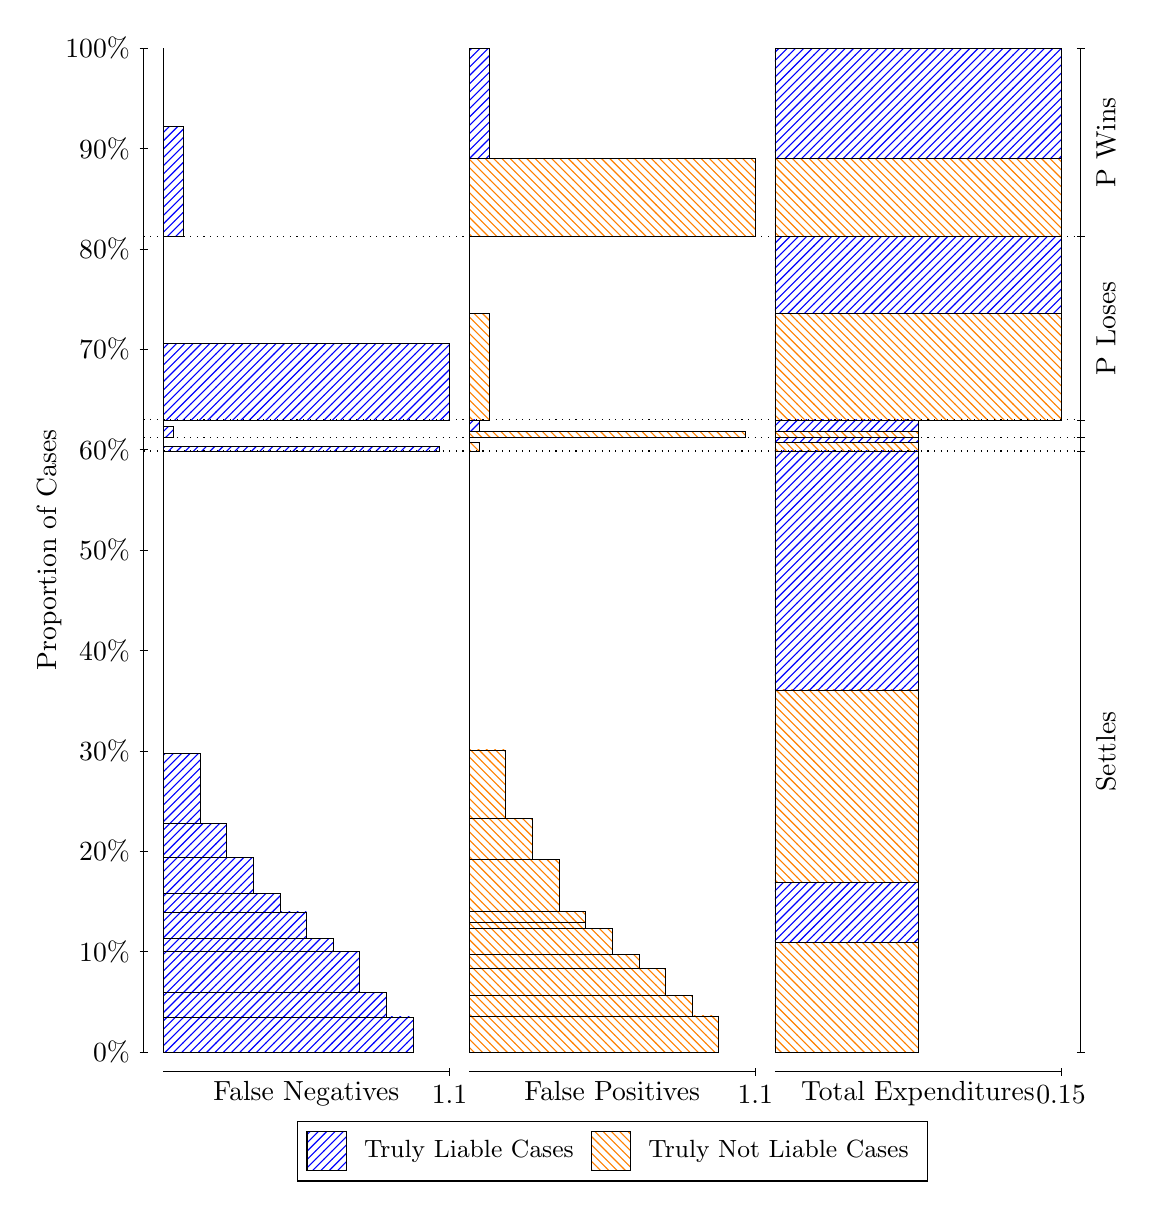
\begin{tikzpicture}
\draw[black, very thin] (1.5,1.75) -- (1.5,14.5);
\node[rotate=90, anchor=center] at (0.3, 8.125) {Proportion of Cases};
\draw[black, very thin] (1.45,1.75) -- (1.55,1.75);
\node[anchor=east] at (1.45, 1.75) {0\%};
\draw[black, very thin] (1.45,3.025) -- (1.55,3.025);
\node[anchor=east] at (1.45, 3.025) {10\%};
\draw[black, very thin] (1.45,4.3) -- (1.55,4.3);
\node[anchor=east] at (1.45, 4.3) {20\%};
\draw[black, very thin] (1.45,5.575) -- (1.55,5.575);
\node[anchor=east] at (1.45, 5.575) {30\%};
\draw[black, very thin] (1.45,6.85) -- (1.55,6.85);
\node[anchor=east] at (1.45, 6.85) {40\%};
\draw[black, very thin] (1.45,8.125) -- (1.55,8.125);
\node[anchor=east] at (1.45, 8.125) {50\%};
\draw[black, very thin] (1.45,9.4) -- (1.55,9.4);
\node[anchor=east] at (1.45, 9.4) {60\%};
\draw[black, very thin] (1.45,10.675) -- (1.55,10.675);
\node[anchor=east] at (1.45, 10.675) {70\%};
\draw[black, very thin] (1.45,11.95) -- (1.55,11.95);
\node[anchor=east] at (1.45, 11.95) {80\%};
\draw[black, very thin] (1.45,13.225) -- (1.55,13.225);
\node[anchor=east] at (1.45, 13.225) {90\%};
\draw[black, very thin] (1.45,14.5) -- (1.55,14.5);
\node[anchor=east] at (1.45, 14.5) {100\%};

\draw[black, very thin] (13.4,1.75) -- (13.4,14.5);
\draw[black, very thin] (13.35,1.75) -- (13.45,1.75);
\node[anchor=west] at (13.35, 1.75) {};
\draw[black, very thin] (13.35,9.3825) -- (13.45,9.3825);
\node[anchor=west] at (13.35, 9.3825) {};
\draw[black, very thin] (13.35,9.5505) -- (13.45,9.5505);
\node[anchor=west] at (13.35, 9.5505) {};
\draw[black, very thin] (13.35,9.7768) -- (13.45,9.7768);
\node[anchor=west] at (13.35, 9.7768) {};
\draw[black, very thin] (13.35,12.104) -- (13.45,12.104);
\node[anchor=west] at (13.35, 12.104) {};
\draw[black, very thin] (13.35,14.5) -- (13.45,14.5);
\node[anchor=west] at (13.35, 14.5) {};

\draw[black, very thin, pattern color=blue, pattern=north east lines] (1.75,1.75) rectangle (4.9186,2.1964);
\draw[black, very thin, pattern color=blue, pattern=north east lines] (1.75,2.1964) rectangle (4.5806,2.5109);
\draw[black, very thin, pattern color=blue, pattern=north east lines] (1.75,2.5109) rectangle (4.2426,3.0235);
\draw[black, very thin, pattern color=blue, pattern=north east lines] (1.75,3.0235) rectangle (3.9047,3.1935);
\draw[black, very thin, pattern color=blue, pattern=north east lines] (1.75,3.1935) rectangle (3.5667,3.5284);
\draw[black, very thin, pattern color=blue, pattern=north east lines] (1.75,3.5284) rectangle (3.2287,3.7596);
\draw[black, very thin, pattern color=blue, pattern=north east lines] (1.75,3.7596) rectangle (2.8907,4.2191);
\draw[black, very thin, pattern color=blue, pattern=north east lines] (1.75,4.2191) rectangle (2.5527,4.6508);
\draw[black, very thin, pattern color=blue, pattern=north east lines] (1.75,4.6508) rectangle (2.2147,5.5455);
\draw[black, very thin, pattern color=orange, pattern=north west lines] (1.75,5.5455) rectangle (1.75,9.3825);
\draw[black, very thin, pattern color=blue, pattern=north east lines] (1.75,9.3825) rectangle (5.2566,9.4403);
\draw[black, very thin, pattern color=orange, pattern=north west lines] (1.75,9.4403) rectangle (1.75,9.5505);
\draw[black, very thin, pattern color=blue, pattern=north east lines] (1.75,9.5505) rectangle (1.8767,9.699);
\draw[black, very thin, pattern color=orange, pattern=north west lines] (1.75,9.699) rectangle (1.75,9.7768);
\draw[black, very thin, pattern color=blue, pattern=north east lines] (1.75,9.7768) rectangle (5.3833,10.746);
\draw[black, very thin, pattern color=orange, pattern=north west lines] (1.75,10.746) rectangle (1.75,12.104);
\draw[black, very thin, pattern color=blue, pattern=north east lines] (1.75,12.104) rectangle (2.0035,13.507);
\draw[black, very thin, pattern color=orange, pattern=north west lines] (1.75,13.507) rectangle (1.75,14.5);
\draw[black, very thin, pattern color=orange, pattern=north west lines] (5.6333,1.75) rectangle (8.8019,2.2097);
\draw[black, very thin, pattern color=orange, pattern=north west lines] (5.6333,2.2097) rectangle (8.464,2.4647);
\draw[black, very thin, pattern color=orange, pattern=north west lines] (5.6333,2.4647) rectangle (8.126,2.8098);
\draw[black, very thin, pattern color=orange, pattern=north west lines] (5.6333,2.8098) rectangle (7.788,2.9901);
\draw[black, very thin, pattern color=orange, pattern=north west lines] (5.6333,2.9901) rectangle (7.45,3.3222);
\draw[black, very thin, pattern color=orange, pattern=north west lines] (5.6333,3.3222) rectangle (7.112,3.391);
\draw[black, very thin, pattern color=orange, pattern=north west lines] (5.6333,3.391) rectangle (7.112,3.5344);
\draw[black, very thin, pattern color=orange, pattern=north west lines] (5.6333,3.5344) rectangle (6.774,4.1935);
\draw[black, very thin, pattern color=orange, pattern=north west lines] (5.6333,4.1935) rectangle (6.436,4.7168);
\draw[black, very thin, pattern color=orange, pattern=north west lines] (5.6333,4.7168) rectangle (6.0981,5.5869);
\draw[black, very thin, pattern color=blue, pattern=north east lines] (5.6333,5.5869) rectangle (5.6333,9.3825);
\draw[black, very thin, pattern color=orange, pattern=north west lines] (5.6333,9.3825) rectangle (5.7601,9.4926);
\draw[black, very thin, pattern color=blue, pattern=north east lines] (5.6333,9.4926) rectangle (5.6333,9.5505);
\draw[black, very thin, pattern color=orange, pattern=north west lines] (5.6333,9.5505) rectangle (9.1399,9.6282);
\draw[black, very thin, pattern color=blue, pattern=north east lines] (5.6333,9.6282) rectangle (5.7601,9.7768);
\draw[black, very thin, pattern color=orange, pattern=north west lines] (5.6333,9.7768) rectangle (5.8868,11.134);
\draw[black, very thin, pattern color=blue, pattern=north east lines] (5.6333,11.134) rectangle (5.6333,12.104);
\draw[black, very thin, pattern color=orange, pattern=north west lines] (5.6333,12.104) rectangle (9.2667,13.096);
\draw[black, very thin, pattern color=blue, pattern=north east lines] (5.6333,13.096) rectangle (5.8868,14.5);
\draw[black, very thin, pattern color=orange, pattern=north west lines] (9.5167,1.75) rectangle (11.333,3.1434);
\draw[black, very thin, pattern color=blue, pattern=north east lines] (9.5167,3.1434) rectangle (11.333,3.9044);
\draw[black, very thin, pattern color=orange, pattern=north west lines] (9.5167,3.9044) rectangle (11.333,6.3479);
\draw[black, very thin, pattern color=blue, pattern=north east lines] (9.5167,6.3479) rectangle (11.333,9.3825);
\draw[black, very thin, pattern color=orange, pattern=north west lines] (9.5167,9.3825) rectangle (11.333,9.4926);
\draw[black, very thin, pattern color=blue, pattern=north east lines] (9.5167,9.4926) rectangle (11.333,9.5505);
\draw[black, very thin, pattern color=orange, pattern=north west lines] (9.5167,9.5505) rectangle (11.333,9.6282);
\draw[black, very thin, pattern color=blue, pattern=north east lines] (9.5167,9.6282) rectangle (11.333,9.7768);
\draw[black, very thin, pattern color=orange, pattern=north west lines] (9.5167,9.7768) rectangle (13.15,11.134);
\draw[black, very thin, pattern color=blue, pattern=north east lines] (9.5167,11.134) rectangle (13.15,12.104);
\draw[black, very thin, pattern color=orange, pattern=north west lines] (9.5167,12.104) rectangle (13.15,13.096);
\draw[black, very thin, pattern color=blue, pattern=north east lines] (9.5167,13.096) rectangle (13.15,14.5);
\draw[black, dotted] (1.5,9.3825) -- (13.4,9.3825);
\draw[black, dotted] (1.5,9.5505) -- (13.4,9.5505);
\draw[black, dotted] (1.5,9.7768) -- (13.4,9.7768);
\draw[black, dotted] (1.5,12.104) -- (13.4,12.104);
\draw[black, very thin] (1.75,1.5) -- (5.3833,1.5);
\node[anchor=north] at (3.5667, 1.5) {False Negatives};
\draw[black, very thin] (5.3833,1.45) -- (5.3833,1.55);
\node[anchor=north] at (5.3833, 1.45) {1.1};

\draw[black, very thin] (5.6333,1.5) -- (9.2667,1.5);
\node[anchor=north] at (7.45, 1.5) {False Positives};
\draw[black, very thin] (9.2667,1.45) -- (9.2667,1.55);
\node[anchor=north] at (9.2667, 1.45) {1.1};

\draw[black, very thin] (9.5167,1.5) -- (13.15,1.5);
\node[anchor=north] at (11.333, 1.5) {Total Expenditures};
\draw[black, very thin] (13.15,1.45) -- (13.15,1.55);
\node[anchor=north] at (13.15, 1.45) {0.15};

\node[black, centered, rotate=90] at (13.72, 5.5662) {Settles};


\node[black, centered, rotate=90] at (13.72, 10.94) {P Loses};
\node[black, centered, rotate=90] at (13.72, 13.302) {P Wins};

\draw (7.449999999999999,1.5) node[draw=none] (baseCoordinate) {};
\begin{scope}[align=center]
        \matrix[scale=0.5, draw=black, below=0.5cm of baseCoordinate, nodes={draw}, column sep=0.1cm]{
            \node[rectangle, draw, minimum width=0.5cm, minimum height=0.5cm, pattern=north east lines, pattern color=blue] {}; &
            \node[draw=none, font=\small] (B) {Truly Liable Cases}; &
            \node[rectangle, draw, minimum width=0.5cm, minimum height=0.5cm, pattern=north west lines, pattern color=orange] {}; &
            \node[draw=none, font=\small] (B) {Truly Not Liable Cases}; \\
            };
\end{scope}

\end{tikzpicture}
\end{document}